% Introdu��o
\chapter{Introdução}
\label{chap:introducao}

Nos últimos oito anos, a busca por termos como \textit{big data} (como pode-se ver na Figura \ref{fig:google-trend}), análise de dados e visualização de dados tem aumentado notoriamente. Existem muitas razões para esse fenômeno, um deles é que com o avanço do poder computacional, precisa-se lidar agora com imensas quantidades de dados, que crescem diariamente, de diversas fontes, em vários formatos e num incrível curto espaço de tempo. Dessa forma, novos desafios vêm surgindo na área de análise de dados: Como processar essas imensas quantidades de dados de forma rápida e eficiente? Como visualizar esse montante de dados? Como \textit{limpar} o conjunto de dados sem perder pontos importantes?

\begin{figure*}[!h]
	\centering
	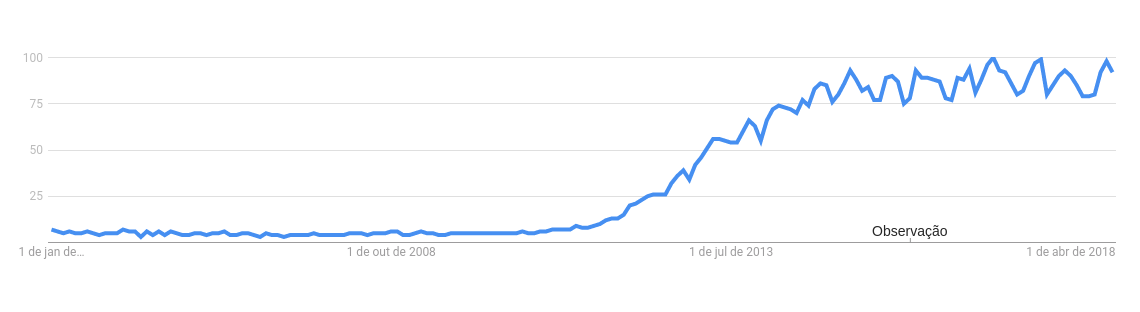
\includegraphics[width=\textwidth]{images/google-trend-big-data.png}
	\caption{Figura retirada do \textit{https://trends.google.com.br} com o resultado do termo \textit{big data}}
	\label{fig:google-trend}
	\vspace{-10pt}
\end{figure*}

No que se refere ao campo da análise de dados, é muito comum que o analista, ao lidar com \textit{datasets} de grandes volumes, encontre, durante sua exploração pelo conjunto de dados, vários pontos com atributos de valores muito distantes da média do dataset no geral, seja distante no sentido de valores muito superiores ou muito inferiores. Isto acontece porque quanto maior é o \text{dataset}, mais facilmente se pode encontrar pontos atípicos que serão mais distantes da distribuição normal. Esse comportamento é importante ser estudado pelo analista para que seja descoberto mais informações sobre o dataset em si e com isso possam ser tomadas decisões mais precisas e afirmações mais claras possam ser propostas. Geralmente, essa preocupação sobre dados anômalos não era tão relevante para a maioria das pesquisas, mas isso vem mudando a partir de que informações importantes podem ser descobertas com essa análise de pontos incomuns. Esse tipo específico de dado com essas características é chamado de Outlier e é muito importante que os atuais analistas de dados deem mais atenção para esses dados, pois informações importantes podem estar escondidas entre esses conjuntos particulares.

Por exemplo, pegando-se um conjunto de dados isolado sobre os fluxo de táxis de Nova Iorque de 2011 e analisando a frequência de corridas no ano inteiro, irão aparecer muitos pontos fora dessa curva média e isso indicaria um comportamento anômalo nessa coleção.

Geralmente, a primeira tarefa a se fazer nessa situação é a remoção desses pontos irregulares e, em seguida, dar continuidade ao processamento no resto do conjunto, mas se levar em consideração outro conjunto de dados isolado sobre a velocidade do vento na região de Nova Iorque nesse mesmo período, poderá-se perceber algum picos de alta velocidade indicando furacões no mesmo momento e na mesma região da queda das corridas de táxi, como apresentado na Figura \ref{fig:freire-paper-taxi-wind}. Análises como essa provam a importância de detectar, estudar e interpretar esse outliers para acrescentar o conhecimento obtido de um dataset.

\begin{figure*}[t]
	\centering
	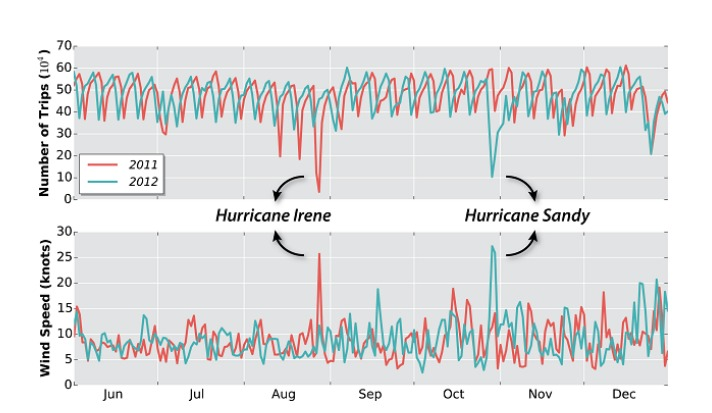
\includegraphics[width=\textwidth]{images/outlier-freire-figure-1}
	\caption{Figura tirada do \cite{DBLP:journals/debu/FreireCVZ16} mostrando a relação entre o número de corridas de táxis e a velocidade do vento}
	\label{fig:freire-paper-taxi-wind}
	\vspace{-10pt}
\end{figure*}

\section{Contextualização}

Hoje em dia as pessoas estão mais e mais conectadas com múltiplas aplicações que acessam um imenso montante dos dados existentes e ainda gera mais dados para melhorar suas análises sobre a sociedade por diversos motivos. Ferramentas como Google Maps\footnote{\it https://maps.google.com}, Uber\footnote{\it https://www.uber.com} e Waze\footnote{\it https://www.waze.com} possuem muitos dados espaciais em tempo real sobre o comportamento dos indivíduos em relação ao tráfego (carros, transporte público, táxis, etc.), local de trabalho, locais de viagem frequentes, etc.

Quando um usuário pretende explorar essas informações, é muito comum que ele se perca frente à tanta massa de dados espaciais e isso vai prejudicar sua possível análise sobre o conjunto, mesmo a mais simples. Esse problema ainda não tem uma solução definitiva, então pesquisas atuais tentam indicar possíveis estratégias para mitigar esse problema e se aproximar de uma solução funcional. Essas abordagens são baseadas em: agrupar um grande conjunto de dados por um ou mais atributos específicos e resumir esses grupos baseado nesses atributos para conseguir simples \textit{insights} sobre esses conjuntos, filtrar o dataset para reduzir os dados visíveis e focar em dados específicos para uma análise mais precisa (mas não vasta), e muitas outras estratégias para reduzir a complexidade da análise.

Junto desses problemas, existe um importante que acontece antes do primeiro passo da análise que é: \textit{O que fazer quando partes do dataset parecem irregular ou com dados corrompidos?} Existem técnicas que ajudam na limpeza dessas partes de forma que não prejudique a análise \cite{10.1007/978-3-319-11116-2_2}, mas estudos recentes demonstram a importância desses dados \textit{``anormais''} e o quanto um analista pode aprender estudando mais precisamente esse conjunto \cite{DBLP:journals/debu/FreireCVZ16}.

Nesse ambiente complexo de análise de dados espaciais com bastante variáveis e possibilidades, um usuário pode facilmente falhar numa dessas tarefas e comprometer seriamente o resultado de suas análises. Combinando todos esses detalhes, sugere-se uma abordagem que leve em consideração o \textit{feedback} do usuário (capturando o movimento do mouse) e, baseado nesse feedback, torne-se apto a analisar o interesse do usuário e dentro disso consiga detectar, estudar e propor ações para serem tomadas quando um dado considerado um outlier apareça nessa região de interesse do usuário.

\section{Objetivos}

Nesta seção estão definidos os objetivos gerais e específicos do trabalho.

\subsection{Objetivos Gerais}

\begin{itemize}
	\item
	      Introduzir o problema da análise e visualização em grandes conjuntos de dados espaciais atualmente.
	\item
	      Explicar a abordagem proposta para detecção de outliers espaciais em grandes datasets utilizando a captura do feedback do usuário e as regiões de sua preferência.
	\item
	      Apresentar os resultados utilizando a proposta para detecção de outliers em um ambiente espaço e os benefícios desse experimento.

\end{itemize}

\subsection{Objetivos Específicos}

\begin{itemize}
	\item
	      Analisar as pesquisas mais recentes na área de detecção de outliers em dados espaço-temporal.
	\item
	      Apresentar uma proposta de ferramenta para análise e visualização de dados espaciais.
	\item
	      Comparar as pesquisas apresentadas destacando os prós e contras de cada pesquisa.
	\item
	      Descrever o conceito de uma região densa interessante utilizado na proposta de ferramenta para mapear a preferência do usuário em um ambiente espacial.
	\item
	      Resumir os algoritmos de detecção de outliers mais conhecidos para dados genéricos e espaciais.
	\item
	      Mostrar o algoritmo escolhido explicando as razões dessa escolha.
	\item
	      Aplicar o conceito de IDR e nosso algoritmo de detecção de outlier escolhido num ambiente de dados espaço-temporal.
	\item
	      Apresentar os resultados da aplicação e indicar trabalhos futuros.

\end{itemize}

\section{Organização do Trabalho}

\abrv[IDR \qquad \textit{Interesting Dense Region}]{}

O documento é organizado do seguinte modo: Capítulo \ref{chap:background} resume as pesquisas existentes no campo da análise e visualização de dados comparando com a ferramenta proposta neste trabalho. Capítulo \ref{chap:outliers} descreve os conceitos de discrepâncias (\textit{outliers}) com os algoritmos existentes para sua detecção, dentre eles o algoritmo escolhido para detectá-las nessa nova proposta. Capítulo \ref{chap:idrs} aborda a concepção de IDR (\textit{Interesting Dense Region}) e como aplicá-las nessa nova abordagem juntamente com a detecção de outliers. Por fim, a conclusão e algumas direções para trabalhos futuros são dados no Capítulo \ref{chap:consideracoes}.